\section{Introduction}

Distributed embedded control systems can be difficult to design due to the heterogeneous 
nature of the domains in which they must operate.  Safety-critical applications also 
require a level of formal verification, to prove to certification authorities (and 
therefore indirectly to the consuming public) that use of these devices entails only 
minimal danger.  

%Model-based design approaches have addressed many of the problems involved in automating 
%embedded systems workflows, but many challenges remain.

Many tools exist to help embedded control system designers assess performance, stability, 
schedulability, and a host of other important properties.  Each of these assessments are 
typically made by analysts trained in either an engineering domain (mechanical, electrical, 
or control design) or in computer science (schedulability, componentization, or deployment 
concerns).  Additionally, each analysis tool may have its own modeling language with distinct 
semantics.  Both situations can lead to inconsistencies in the understanding of the design.

In current practice, much of the reconciliation of design discrepancies is still done by 
hand.  Design inconsistencies are discovered by individual designers or in review meetings.  
Manual reconciliation of issues occurs as individual designers receive assignments to modify 
and correct the design.

%Differences that prove to be too costly to rework end up being worked around.
% Fig. \ref{fig:integration} provides a glimpse into the diversity and multitude of analyses frequently involved. 

Supporting such heterogeneity of analysis tools and domains requires everyone involved in 
the design process to have a consistent view of design details.  Reconciling semantics 
between formalisms and tools is costly and time-consuming.  Often the effort can not be 
justified outside of academic research unless the results are applicable to numerous designs.

%\begin{figure}
%\centering
%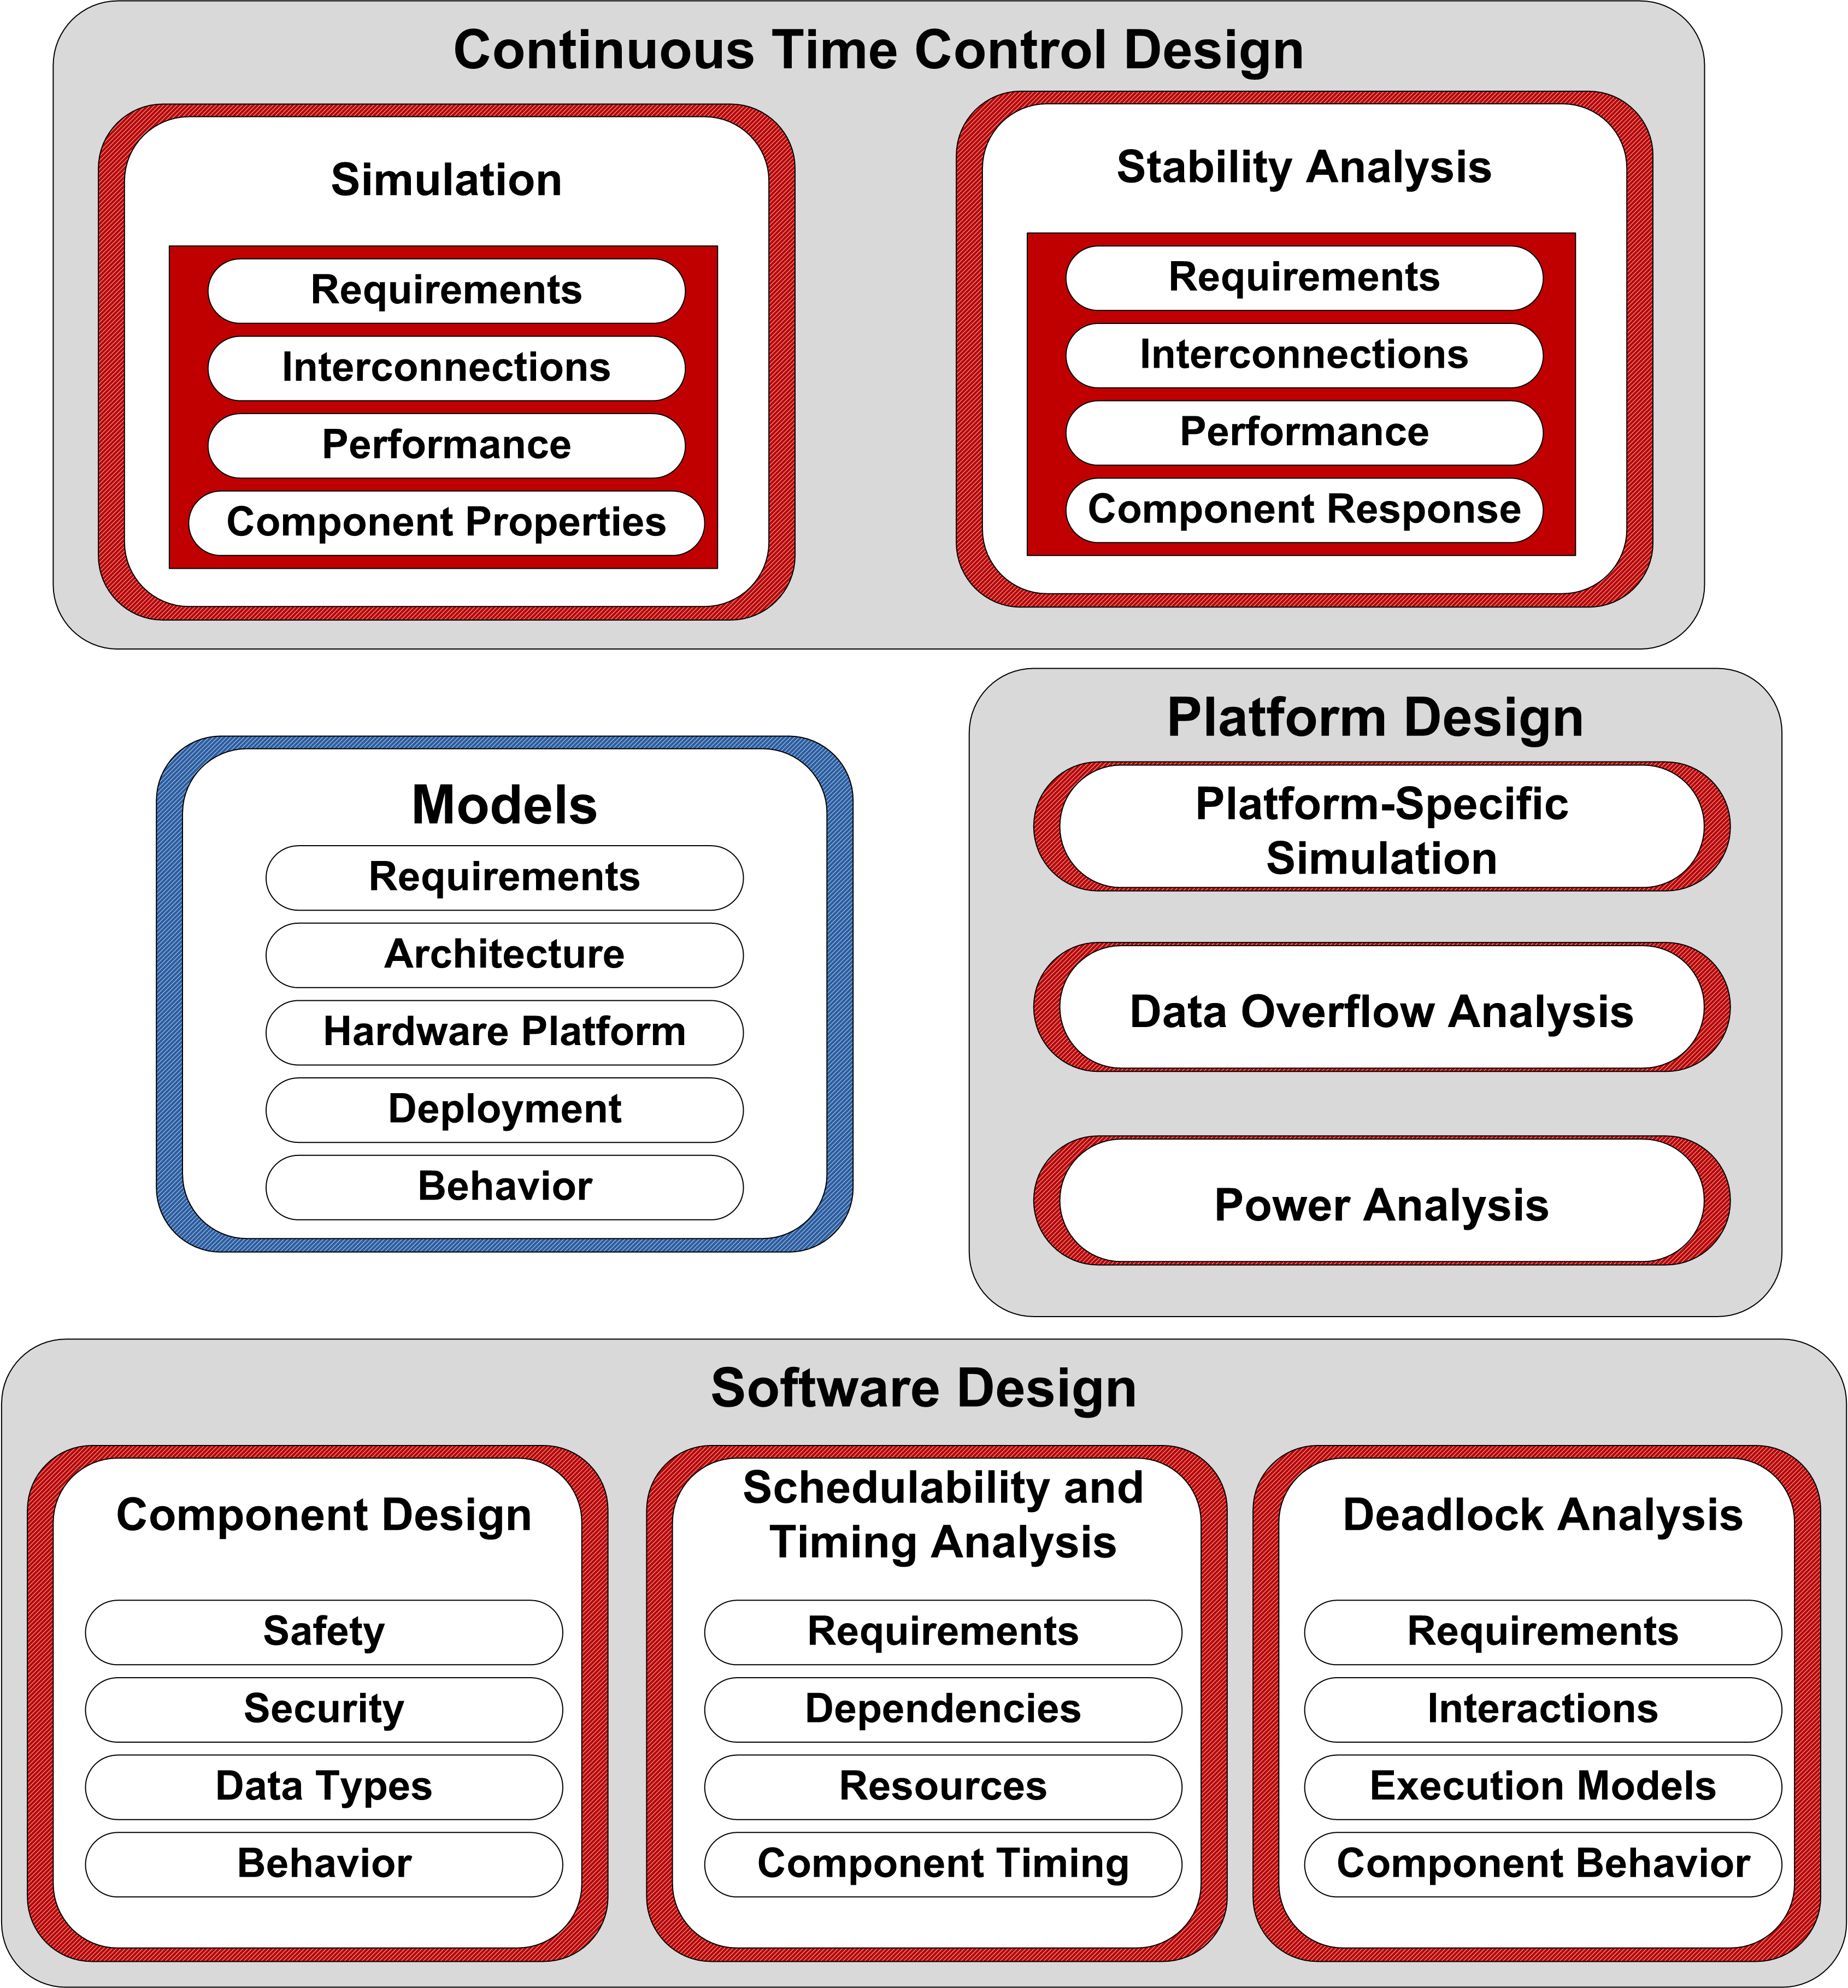
\includegraphics[width=\columnwidth]{figures/analysis_integration.png}
%    \caption{Conceptual illustration of the analysis integration problem. Proper mapping of structural and behavioral details from each of the analysis domains to the modeling environment facilitates a consistent view of the design during development.}
%    \label{fig:integration}
%\end{figure}

In the model integrated computing approach, domain specific modeling languages represent 
different aspects of the design, with the promise of consistently integrating different tools 
and techniques.  We present here a sketch of a formal model-based approach which promises to tame 
many of the difficulties involved in consistently integrating heterogeneous analysis tools into a 
single workflow.  Our approach can be considered as an implementation of the tool integration ideas 
in \cite{modeling:hybrid_abs}, but with variations of the details included in the design language.  
Specifically we propose six main ideas:

\begin{itemize}

\item A front end graphical modeling language which integrates into existing embedded design 
workflows\cite{modeling:aces08}\cite{sched:analysis}.

\item A single transformation from front end models to an intermediate language explicitly 
representing a flattened semantic model, including parameters and objects to imply a precise 
(unambiguous, analyzable, and executable) behavioral semantics.  We differ from the approach 
in \cite{modeling:hybrid_abs} by abstracting the dynamic behavior using passive control design 
techniques. We rely on the resulting robustness and compositionality of the passive approach 
to simplify design analysis and implementation.

\item Both the front-end and intermediate languages support platform-based design \cite{modeling:platform}, 
separating component-level concerns and interaction concerns where possible.

\item Generation of analysis models from the intermediate language using simple template generation techniques.

\item Representation of structural and behavioral concepts from the intersection of the semantic 
domains of the analysis tools as primitives in the front end language.

\item Round-trip incorporation of calculated analysis results into the modeling environment to 
maintain consistency as models pass between design phases.

\end{itemize}

The described approach is part of the ESMoL modeling language and embedded software design 
suite\cite{modeling:aces08}.  ESMoL is a research experiment in the implementation of modeling 
tools to support compositional analysis and design frameworks.  In our design flow a modeler 
imports Simulink/Stateflow models \cite{tools:mathworks} into the ESMoL language, adds architecture 
elements, platform design, and deployment concepts, then performs automated analysis and synthesizes 
code for execution on a time-triggered platform\cite{timed:tta}.  We aim to support iterative development, 
as analysis data can flow back to earlier stages for re-design or re-evaluation.  The language and tools 
also include preliminary support for requirements modeling, by allowing specification of maximal latency 
bounds between computational tasks in the design.
